\section{Login and Registration}

\begin{figure}[hb]
	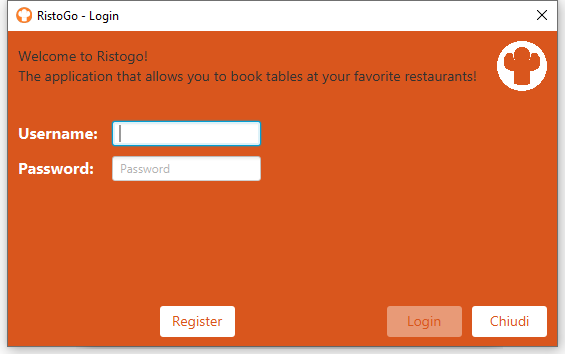
\includegraphics[width=\textwidth]{login}
	\caption{Login interface.}
	\label{fig:login}
\end{figure}

When the application starts it opens the main page (Figure~\ref{fig:login}), on
which an old user can insert username and password to login, clicking on the
button ``Login''.

Otherwise, if the user is a new one, he must do the registration procedure to
use the application.

If you want to close the application, click on the button ``Close''.

\subsection{Registration}

If you are a new user, click on ``Register'' on the main page to open the
registration form (Figure~\ref{fig:customerregistration}).

Then, insert your username and your password (the password must contain at least
8 characters). Insert another time your password to confirm and, in the section
``type of user'', select \code{Customer} if you want to use the application for
book tables or select \code{Owner} if you want to insert your restaurant in the
application to manage its reservations (Figure~\ref{fig:ownerregistration}).

If you went in the registration page wrongly, click on ``Login'' to return to
the login page.

\begin{figure}[ht]
	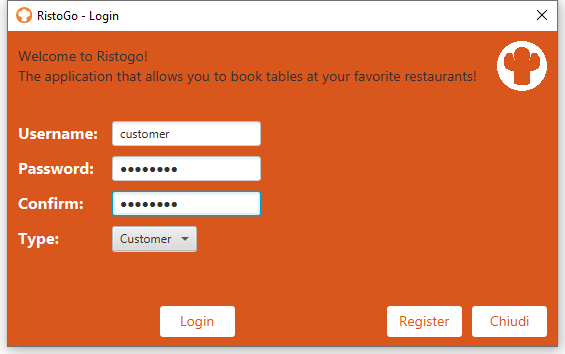
\includegraphics[width=\textwidth]{customerregistration}
	\caption{Registration of a Customer user.}
	\label{fig:customerregistration}
\end{figure}

\begin{figure}[ht]
	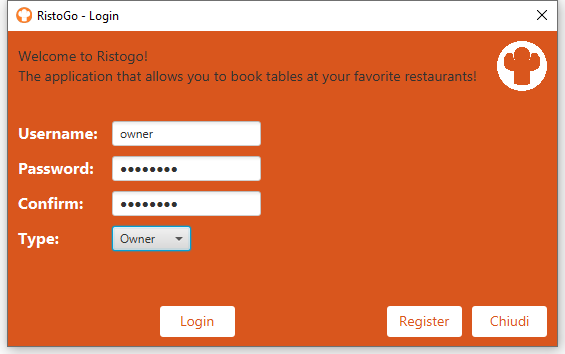
\includegraphics[width=\textwidth]{ownerregistration}
	\caption{Registration of a Owner user.}
	\label{fig:ownerregistration}
\end{figure}

When you filled out the form, click on ``Register''. Now if you don’t receive
error messages your account will be create. So you can start to use the
application for the first time.
